\chapter{Kalor dan Isolasi}\label{ch:g5:heat-and-insulation}

Mengapa perosotan logam terasa sedingin es sementara bangku kayu di
sebelahnya tidak? Teka-teki itu membuntuti kita sejak tahun pertama
buku ini. Hari ini ia jatuh --- bersama rahasia termos, jendela ganda,
dan burung pipit yang menggembung pada \omterm{def:g3:sun-days-seasons:year}{musim} dingin. Kuncinya adalah
berhenti bertanya bagaimana benda \emph{terasa} dan mulai mengikuti ke
mana \omterm{def:g5:heat-and-insulation:heat}{kalor} \emph{mengalir}.

\section{Kalor sedang bergerak}

\begin{definition}[Kalor]\label{def:g5:heat-and-insulation:heat}
Yang disebut \emph{kalor}\index{kalor} adalah \omterm{def:g5:everyday-energy:energy}{energi} yang sedang
berpindah dari benda yang lebih panas ke benda yang lebih dingin. Sup
menyerahkan kalor kepada sendok, radiator kepada ruangan, tanganmu
kepada bola salju. Kalor bukanlah zat yang bersembunyi di dalam benda
panas --- ia adalah sebuah \emph{aliran}, dan ia selalu punya arah.
\end{definition}

\begin{proposition}[Kalor mengalir menurun]\label{prop:g5:heat-and-insulation:downhill}
Dengan sendirinya, \omterm{def:g5:heat-and-insulation:heat}{kalor} selalu mengalir dari benda yang lebih panas
ke benda yang lebih dingin --- tidak pernah sebaliknya. Alirannya
berjalan selama kedua \omterm{def:g3:temperature-thermometers:temperature}{suhunya} berbeda, dan mereda ketika keduanya
bertemu: kalau dibiarkan bersama cukup lama, tetangga yang panas dan
yang dingin berakhir pada satu \omterm{def:g3:temperature-thermometers:temperature}{suhu} yang sama.
\end{proposition}

\begin{example}[Membaca arahnya]\label{ex:g5:heat-and-insulation:direction}
Sendok teh di dalam teh menjadi panas: \omterm{def:g5:heat-and-insulation:heat}{kalor} mengalir teh $\to$
sendok. Limun berbongkah es menjadi dingin --- hati-hati! Tidak ada
sesuatu bernama ``dingin'' yang mengalir masuk: \omterm{def:g5:heat-and-insulation:heat}{kalor} mengalir
\emph{keluar dari limunnya ke dalam esnya}, lalu mencairkannya. Dingin
bukanlah sebuah aliran; ia hanya nama yang kita berikan kepada pihak
yang kalah. Buku fisika semuanya menulis ``minumannya kehilangan
\omterm{def:g5:heat-and-insulation:heat}{kalor}'', tidak pernah ``minumannya mendapat dingin''.
\end{example}

\begin{omfigure}
\begin{tikzpicture}[scale=0.85]
  \draw[thick] (0.6,0.4) rectangle (3.0,1.9);
  \node[font=\small] at (1.8,1.15) {sup panas};
  \draw[thick] (7.8,0.4) rectangle (10.2,1.9);
  \node[font=\small] at (9.0,1.15) {udara sejuk};
  \draw[-Stealth, line width=3pt, omThm] (3.3,1.15) -- (7.5,1.15);
  \node[above, font=\small, omThm] at (5.4,1.4)
    {kalor mengalir panas $\to$ dingin};
  \node[below, font=\small] at (5.4,0.0)
    {dan berhenti hanya ketika kedua suhunya bertemu};
\end{tikzpicture}

{\small Satu aturan untuk setiap dapur dan setiap \omterm{def:g3:sun-days-seasons:year}{musim} dingin: \omterm{def:g5:heat-and-insulation:heat}{kalor}
berlari menurun, dari yang lebih panas ke yang lebih dingin, sampai
bukitnya habis.}
\end{omfigure}

\section{Jalur cepat dan jalur lambat}

\begin{definition}[Konduktor dan isolator kalor]\label{def:g5:heat-and-insulation:conductors}
Setiap zat sangat berbeda dalam hal secepat apa ia membiarkan \omterm{def:g5:heat-and-insulation:heat}{kalor}
mengalir melewatinya. Sebuah
\emph{konduktor kalor}\index{konduktor kalor} adalah jalur cepat ---
logam di atas segalanya. Sebuah
\emph{isolator kalor}\index{isolator kalor} adalah jalur lambat: kayu,
wol, plastik, bulu --- dan sang juara, \emph{\omterm{def:g2:air-around-us:air}{udara} yang diam}, yang
terperangkap sehingga tidak dapat berpusar. (Kedua kata itu dipinjam
dengan sengaja dari \omterm{def:g4:conductors-insulators:conductor}{konduktor} dan \omterm{def:g4:conductors-insulators:insulator}{isolator} listrik; kedua sifat itu
sering, tetapi tidak selalu, berjalan bersama.)
\end{definition}

\begin{omfigure}
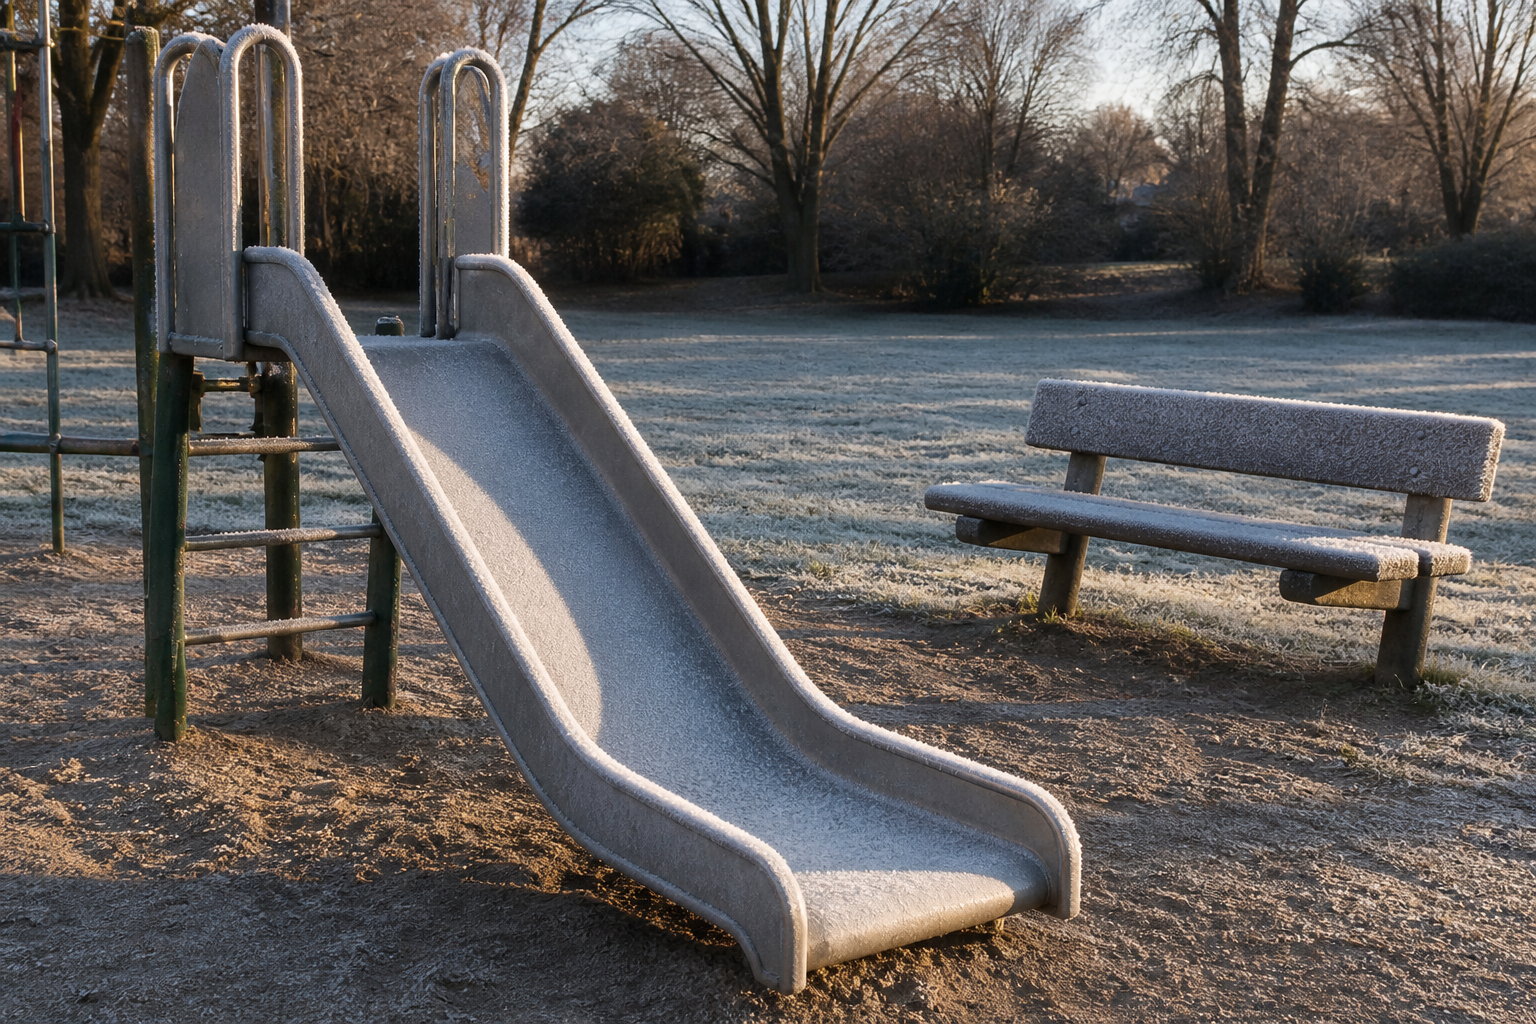
\includegraphics[width=0.58\linewidth]{images/book1/ai/g5-heat-frosty-slide.png}

{\small Pagi yang berembun beku di halaman bermain: perosotan logam dan bangku kayu melewati malam yang sama pada \omterm{def:g3:temperature-thermometers:temperature}{suhu} yang sama --- namun hanya salah satunya yang akan menggigit kulitmu.}
\end{omfigure}

\begin{example}[Teka-teki perosotan, terpecahkan]\label{ex:g5:heat-and-insulation:slide}
Perosotan logam dan bangku kayu melewati malam pada \omterm{def:g3:temperature-thermometers:temperature}{suhu} dingin yang
sama --- \omterm{def:g3:temperature-thermometers:temperature}{termometer} sudah bersumpah begitu sejak lama. Sentuhlah
keduanya: tanganmu lebih hangat daripada keduanya, sehingga \omterm{def:g5:heat-and-insulation:heat}{kalor}
mengalir darimu ke masing-masingnya. Tetapi logamnya jalur cepat ---
ia menyapu kalormu pergi dengan terburu, dan \emph{keterburuan} itulah
yang terasa sebagai ``sedingin es''. Kayunya mengambil kalormu hanya
setetes demi setetes: nyaris tidak terasa sejuk. Kulitmu tidak pernah
\omterm{def:g2:measuring-length:measure}{mengukur} \omterm{def:g3:temperature-thermometers:temperature}{suhu} --- ia \omterm{def:g2:measuring-length:measure}{mengukur} laju kehilangan \omterm{def:g5:heat-and-insulation:heat}{kalornya} sendiri.
Perkaranya ditutup, sesudah empat tahun.
\end{example}

\begin{method}[Lomba mendingin]\label{met:g5:heat-and-insulation:race}
Saksikan isolasi menang, dengan bilangan:
\begin{enumerate}
  \item isilah dua cangkir yang serupa dengan air keran yang sama
        panasnya (\emph{mintalah orang dewasa memberi air hangat
        setangan, bukan air mendidih});
  \item bungkuslah satu cangkir tebal-tebal dengan syal wol; biarkan
        yang lain telanjang;
  \item tancapkan \omterm{def:g3:temperature-thermometers:temperature}{termometer} di masing-masingnya lalu tulislah kedua
        \omterm{def:g3:temperature-thermometers:temperature}{suhunya} dalam sebuah tabel setiap lima menit, enam kali;
  \item gambarlah kedua catatan itu sebagai dua garis pada satu
        grafik, \omterm{def:g3:temperature-thermometers:temperature}{suhu} terhadap waktu.
\end{enumerate}
Garis cangkir yang telanjang menukik; garis cangkir yang terbungkus
melandai lembut. Awal yang sama, ruangan yang sama --- wolnya membuat
pintu keluar \omterm{def:g5:heat-and-insulation:heat}{kalor} menjadi jalur lambat.
\end{method}

\begin{omfigure}
\begin{tikzpicture}
\begin{axis}[omaxis, width=10.5cm, height=5.6cm,
    xlabel={menit}, ylabel={suhu (\unit{\celsius})},
    xtick={0,5,10,15,20,25,30}, ytick={20,30,40,50},
    ymin=15, ymax=55, xmin=-1, xmax=31]
  \addplot[very thick, omDef] coordinates
    {(0,50) (5,46.5) (10,43.5) (15,41) (20,39) (25,37.5) (30,36)};
  \addplot[very thick, omThm] coordinates
    {(0,50) (5,41) (10,34.5) (15,30) (20,27) (25,24.5) (30,23)};
  \node[right, font=\small, omDef] at (axis cs:24,39.5)
    {terbungkus wol};
  \node[right, font=\small, omThm] at (axis cs:19,25.5) {cangkir telanjang};
\end{axis}
\end{tikzpicture}

{\small Lomba mendingin, digambar: dua cangkir air \qty{50}{\celsius}
di ruangan \qty{20}{\celsius}. Wolnya tidak dapat menghentikan
pelarian \omterm{def:g5:heat-and-insulation:heat}{kalor} --- tetapi ia memperlambatnya dengan indah.}
\end{omfigure}

\begin{remark}[Isolasi hanya memperlambat]\label{rem:g5:heat-and-insulation:onlyslows}
Perhatikan ke mana kedua kurvanya menuju: ke arah \qty{20}{\celsius}
milik ruangan itu. Tidak ada syal, tidak ada termos, tidak ada dinding
iglo yang pernah menghentikan aliran menurun \omterm{def:g5:heat-and-insulation:heat}{kalor} --- isolasi hanya
membuat jalur lambatnya lebih lambat lagi. Itu pula sebabnya mantel
pada manusia salju (ingat dia?) menunda pencairannya tetapi tidak
dapat menyelamatkannya: \omterm{def:g5:heat-and-insulation:heat}{kalor} \omterm{def:g3:sun-days-seasons:year}{musim} panas tetap merembes masuk.
\end{remark}

\section{Seni memerangkap udara}

\begin{example}[Rekayasa musim dingin]\label{ex:g5:heat-and-insulation:air}
Hampir setiap benda penghangat yang kamu miliki adalah mesin untuk
memerangkap \omterm{def:g2:air-around-us:air}{udara}. Wol menghangatkanmu bukan oleh seratnya sendiri
melainkan oleh kantong \omterm{def:g2:air-around-us:air}{udara} yang tak terhitung banyaknya di
antaranya; selimut bulu, kain bulu domba, dan burung pipit yang
menggembung menjadi bola di kawat yang \omterm{def:g2:ice-water-steam:meltfreeze}{membeku} semuanya memainkan
kartu yang sama. Rumah ikut bergabung: jendela ganda memenjarakan
selapis \omterm{def:g2:air-around-us:air}{udara} di antara dua kaca, dan dinding berisolasi diisi
sumpalan halus yang menimbun \omterm{def:g2:air-around-us:air}{udara}. \omterm{def:g2:air-around-us:air}{Udara} yang diam adalah jalur
lambat sang juara --- tipuannya adalah menjaga \omterm{def:g2:air-around-us:air}{udaranya} tetap
\emph{diam}.
\end{example}

\begin{example}[Termos]\label{ex:g5:heat-and-insulation:thermos}
Botol termos adalah mahakarya isolasi: sebuah botol di dalam botol,
dengan \omterm{def:g2:air-around-us:air}{udara} di antara keduanya dipompa keluar sampai hampir tidak ada
--- dan di tempat yang hampir tidak berisi zat, aliran \omterm{def:g5:heat-and-insulation:heat}{kalor} hampir
tidak menemukan jalur sama sekali (tipuan yang layak diingat:
kekosongan yang sama pernah membungkam lonceng di dalam toples).
Tambahkan dinding yang mengkilap untuk memantulkan pijar kehangatan
kembali ke dalam, dan cokelat panas menemui sore hari dalam keadaan
masih panas --- atau limun masih dingin: termos tidak tahu apa-apa
tentang panas atau dingin, ia hanya menutup jalurnya, ke dua arah.
\end{example}

\begin{remark}[Cara menghangatkan diri, dikatakan dengan benar]\label{rem:g5:heat-and-insulation:coat}
Sekarang pertanyaan mantel yang lama tertutup untuk selamanya. Mantel
adalah \omterm{def:g2:air-around-us:air}{udara} yang terperangkap di sekeliling sebuah pembuat \omterm{def:g5:heat-and-insulation:heat}{kalor} ---
yaitu kamu. Tubuhmu mengalirkan \omterm{def:g5:heat-and-insulation:heat}{kalor} keluar sepanjang hari; mantel
mengubah aliran itu menjadi rembesan, dan kamu tetap hangat dengan
produksimu sendiri. Pada manusia salju --- yang tidak punya pembuat
\omterm{def:g5:heat-and-insulation:heat}{kalor} di dalamnya --- mantel yang sama sekadar memperlambat rembesan
\omterm{def:g3:sun-days-seasons:year}{musim} panas yang masuk. Isolasi tidak pilih kasih: ia memperlambat
alirannya, ke arah mana pun aliran itu berjalan.
\end{remark}

\section{Latihan}

\begin{exercise}[$\star$]\label{exo:g5:heat-and-insulation:1}
Apa itu \omterm{def:g5:heat-and-insulation:heat}{kalor}, dan ke arah mana ia mengalir dengan sendirinya? Kapan
alirannya berhenti?
\end{exercise}

\begin{exercise}[$\star$]\label{exo:g5:heat-and-insulation:2}
``Tutup pintunya, kamu membiarkan dinginnya masuk!'' Tulislah ulang
kalimat nenek itu sebagaimana buku fisika menuliskannya.
\end{exercise}

\begin{exercise}[$\star$]\label{exo:g5:heat-and-insulation:3}
Pilahlah menjadi jalur cepat dan jalur lambat bagi \omterm{def:g5:heat-and-insulation:heat}{kalor}: panci
tembaga; \ syal wol; \ sendok baja; \ \omterm{def:g2:air-around-us:air}{udara} yang diam; \ sendok kayu;
\ selimut bulu.
\end{exercise}

\begin{exercise}[$\star$]\label{exo:g5:heat-and-insulation:4}
Mengapa panci berdasar logam tetapi bergagang plastik atau kayu?
Jawablah dengan jalur.
\end{exercise}

\begin{exercise}[$\star$]\label{exo:g5:heat-and-insulation:5}
Akhirnya, dengan kata-katamu sendiri: mengapa logam terasa lebih
dingin daripada kayu pada \omterm{def:g3:temperature-thermometers:temperature}{suhu} yang sama? Apa yang sebenarnya diukur
kulit?
\end{exercise}

\begin{exercise}[$\star$]\label{exo:g5:heat-and-insulation:6}
Pada lomba mendingin, mengapa kedua cangkirnya harus serupa dan mulai
sama panasnya? Satu perbedaan apa yang sedang diuji percobaan itu?
\end{exercise}

\begin{exercise}[$\star$]\label{exo:g5:heat-and-insulation:7}
Bacalah grafik pendinginannya: kira-kira berapa \omterm{def:g3:temperature-thermometers:temperature}{suhu} yang ditunjukkan
tiap cangkir sesudah $15$ menit? Menuju \omterm{def:g3:temperature-thermometers:temperature}{suhu} berapa kedua kurvanya
mengarah, dan mengapa?
\end{exercise}

\begin{exercise}[$\star$]\label{exo:g5:heat-and-insulation:8}
Mengapa burung pipit menggembungkan dirinya menjadi bola di kawat yang
\omterm{def:g2:ice-water-steam:meltfreeze}{membeku}? Sebutkan tiga temuan manusia yang memainkan kartu yang sama.
\end{exercise}

\begin{exercise}[$\star\star$]\label{exo:g5:heat-and-insulation:9}
Termos yang sama menjaga cokelat tetap panas pada bulan Januari dan
limun tetap dingin pada bulan Juli. Jelaskan bagaimana satu alat
sanggup melakukan kedua pekerjaan itu --- apa sebenarnya yang
dilakukan termos, dan terhadap apa?
\end{exercise}

\begin{exercise}[$\star\star$]\label{exo:g5:heat-and-insulation:10}
Seorang penjual es krim membungkus wadahnya dengan selimut wol tebal
pada hari yang panas, dan seorang pembeli tertawa: ``Wol itu untuk
menjaga benda tetap hangat!'' Belalah penjualnya dengan
\cref{rem:g5:heat-and-insulation:coat} --- ke arah mana \omterm{def:g5:heat-and-insulation:heat}{kalor} sedang
mencoba mengalir, dan apa yang dilakukan wolnya terhadapnya?
\end{exercise}

\begin{exercise}[$\star\star$]\label{exo:g5:heat-and-insulation:11}
Dua rumah berdiri pada \omterm{def:g3:sun-days-seasons:year}{musim} dingin yang sama: satu berjendela
tunggal, satu berjendela ganda. Jelaskan dengan jalur dan \omterm{def:g2:air-around-us:air}{udara} yang
terperangkap mengapa rumah berjendela ganda membakar lebih sedikit
bahan bakar --- dan mengapa, menurut
\cref{rem:g5:heat-and-insulation:onlyslows}, ia tetap memerlukan
pemanasan \emph{sedikit}.
\end{exercise}
